\documentclass[a4paper, 11pt, titlepage]{report}

\usepackage[margin=2.0cm]{geometry}

\usepackage{xspace}
\def \itwoc {I\textsuperscript{2}C\xspace}
\def \vdd {V\textsubscript{DD}}

% Indent the first line of the first paragraph like the first lines of subsequent paragraphs
\usepackage{indentfirst}

% Don't indent any first lines
\setlength{\parindent}{0mm}

% A little space between paragraphs
\setlength{\parskip}{1.5mm}

% Display
% 1. <chapter title>
% instead of
% Chapter 1
% <chapter title>
\makeatletter
\renewcommand{\@makechapterhead}[1]{%
\vspace*{50 pt}%
{\setlength{\parindent}{0pt} \raggedright \normalfont
\bfseries\Huge\thechapter.\ #1
\par\nobreak\vspace{40 pt}}}
\makeatother

% In order to include images
\usepackage{graphicx}

% Label figures 1, 2, 3, 4... Instead of 1.1, 1.2, 2.1, 3.1 etc.
\usepackage{chngcntr}
\counterwithout{figure}{chapter}

% Display SI units
\usepackage[separate-uncertainty=true, multi-part-units=single]{siunitx}

% To have text wrapped around images
\usepackage{wrapfig}

% Some parameters for wrapfig
\setlength{\intextsep}{0pt}%
\setlength{\columnsep}{15pt}%

% Same as regular math but with a bit of space before and after
\newenvironment{ownmath}
{\vspace{2mm}\hspace{15pt}\begin{math}}
{\end{math}\vspace{2mm}}










\begin{document}

\title{Development of a 3D display}
\author{Balduin Dettling}

% Generate title
\maketitle

% Introduction
% * after chapters to not number them
% TODO: don't show page numbers
\chapter*{Preface}

\pagenumbering{Roman}

\section*{Motivation}

For as long as I can remember, I've been fascinated by all kinds of technology.
It was clear to me that my final thesis would be a practical one in the field of engineering.
However, I didn't have anything specific in mind for quite some time.

One day, I stumbled upon a project report on the internet about a so-called persistence of
vision display. It was a simple row of LEDs, driven by a microcontroller, and mounted on an
electric motor. The contraption was (and presumably still is) able to draw images into the
air by precisely controlling the row of LEDs. Fascinated by this, I did some research and
found that a plethora of similar projects exists, some even with detailed instructions on how
to build the device in question.

I had the idea of building several rows of LEDs and arranging them on top of each other.
That way, I could display several two-dimensional bitmap images above another, resulting in a
three-dimensional image.

Having had no previsous experience in the field of electronics, it seemed a bit daunting to
build a 3D display. I could, however, motivate myself to attempt it anyway by telling myself
that the project wouldn't be much more complex than all of the 2D versions out there (which
turned out to be not very far from the truth).


\section*{Credits}

First and foremost, I would like to express my gratitude to Mr. Patrick Spengler, my physics
teacher and the mentor of this thesis. Not only did he solve numerous malfunctions, but he also
is partly responsible for my interest in electronics and engineering.

I am thankful to Ms. Ursula Schamberger, teacher of the woodworking class, where I built the
wooden frame. Likewise, I would like to thank Mr. Hanspeter Rieder, who kindly granted me
access to the school's electronics workshop.

Last, but most certainly not least, I am indebted to Prof. Heinz Domeisen. He mentored the
advancement and refinement of the thesis in preparation for the national competition organised
by "Swiss Youth in Science".

\section*{Declaration of authorship}

I hereby declare that the following thesis has been authored entirely by myself, Balduin
Dettling, and confirm that all external sources of information are cited correctly.

\vspace{10mm}
\rule{\textwidth}{0.5pt}
\begin{minipage}[t]{0.5\textwidth}
Location and Date
\end{minipage}
\begin{minipage}[t]{0.5\textwidth}
\hspace{-1mm}Signature
\end{minipage}


% Generate table of contents
\tableofcontents



\chapter{Introduction}

\pagenumbering{arabic}

\section{Current State of The Art}

% todo: references
As discussed before, there is no shortage of projects that are similar to mine, but only
display 2D images. The name "POV display", short for persistence of vision display, has become
commonplace. Another popular name is "Propeller Clock" --- Propeller because it rotates like one,
and clock because the round shape is ideal for displaying an analog clock.

As far as I know, however, only two people have built a working version of a three-dimensional
POV display so far (and have published it on the internet).\footnote{It turned out that there was
a third one: When I posted a picture of my project on the internet, a reddit user told me about
the display he built years before.}
Neither of these is being produced on a grand scale, instead they are --- like most 2D versions
--- side projects of hobbyists or engineers.

\section{Goals}

The objective of this project is to build a working prototype of a 3D persistence of vision
display and to document the process of doing so. The necessary steps are (roughly) as follows:

\begin{itemize}
\item Understand and explain how and why such a display can work in principle
\item Come up with realistic technical specifications, founded on the previously outlined
theory
\item Select parts and build the device according to the specifications
\item Write a program that makes the device display a 3D image
\item Draw conclusions: Did I achieve my goals? What could have been done better?
How can the project be further improved?
\end{itemize}





\chapter{Theory and Planning}

\section{Principle of Operation}

\subsection{Persistence of Vision}

Persistence of Vision refers to the optical illusion that results whenever the image we look
at quickly changes. In such situations, we don't immediately see the new image, instead we
continue seeing the old image for a short timespan after it has vanished. If wikipedia is to
be believed, this timespan is about $\frac{1}{25}$ of a second, but of course it is going to
be different for each pair of eyes.

Although we don't normally see this effect in action, there are situations where it becomes
apparent. For example, if a car drives by at nighttime, we see traces of light behind the
actual car lights for a short moment (Assuming our eyes don't follow the car and stay still
relative to the environment). In general, bright flashes of light followed by (relative)
darkness tend to be the most pronounced manifestation of persistence of vision. It is exactly
this situation that can be recreated and exploited for the successful operation of a persistence
of vision display.

\subsection{Exploiting Persistence of Vision}

Normally, Persistence of Vision is nothing more than an interesting effect. However, we can
use this weakness of the human eye to our benefit.

If a light source is spun quickly enough in a circle, we don't see a spinning
point anymore, but instead we see one solid circle. This is because the rotational period is
shorter than the time it takes for the light to fade away on our retinas. The rotational period
at which we stop seeing a flickering circle and start seeing a solid, still circle is called
the flicker fusion threshold.

By controlling this light source quickly and accurately, we can make it so it is always turned
on at certain points in the circle, and always turned off at others. By doing so, we are
effectively multiplexing a zero-dimensional display (a point-like light source, e.g. an LED)
so that it displays a one-dimensional image. By rotating a whole row of LEDs (a one-dimensional
display), we can display two-dimensional images. Finally, if there are multiple rows of LEDs
that together form a two-dimensional display, it is possible to display a three-dimensional
image.


\section{Specifications}

\begin{itemize}

\item Resolution of $16 \cdot 100 \cdot 10$ pixels (radius $\cdot$ circumference $\cdot$ height)
\item Each pixel consists of an RGB LED
\item Colour depth of 3 bit per pixel, or one bit per LED
\item Rotational frequency of at least 30 Hz, or as fast as it needs to be in order to not flicker

\end{itemize}




\section{Components}

\subsection{Control}

For controlling the LEDs, I have bought a Teensy 3.1 microcontroller development board. It has a
small footprint --- ideal for the fast rotation --- and still packs quite some power: The processor
runs at 96 MHz at a register width of 32 bit. There are 34 configurable I/O pins.

The controller has to have some kind of reference point, so that it can calculate the current speed
and angular position of the device. For this, I used a simple hall sensor on the rotating side,
which passes by a stationary magnet after each rotation.



\subsection{Data Transmission}

34 I/O pins are quite a lot, but not quite enough to directly control 480 LEDs. In order to still
access all those LEDs individually, I had to use LED drivers. These come in the form of integrated
circuits and receive some amount of data that they use to control a corresponding amount of LEDs.

Initially, I had planned to implement a colour depth of 8 bits, allowing for
$2^{24} = 16777216$ different colours. However, there were several difficulties that I would have
had to deal with. First of all, all of the available LED drivers had one or both of the following
shortcomings:

\begin{itemize}

\item Controlled using \itwoc  instead of SPI

Because \itwoc uses pullup resistors instead of a push-pull drive, it takes a little moment for
the logic level to return to its normal state. In order to ensure correct data transmission, it is
necessary to set a relatively slow clock speed. The two \itwoc interfaces of the Teensy only
support clock speeds of up to 2.4 MHz --- and because \itwoc requires some overhead data to send
out the slave's addresses, the actual data rate will be even lower.

However, the minimum data rate required to control the LEDs at an 8-bit colour depth is as follows:

\begin{ownmath}
% Yes it's a mess but \si makes it a unit, so it is not in cursive while still being small enough
24\,\frac{\si{bit}}{\si{pixel}} \cdot 16000\,\frac{\si{pixels}}{\si{rotation}} \cdot
30\,\frac{\si{rotations}}{\si{second}} = \SI{11.52}{Mbps}
\end{ownmath}

This means that I'd need at least 5 parallel \itwoc lines to control all the LEDs with 8 bit colour
depth. Because each Teensy only has two of them, I'd need three Teensy boards, which would be
possible but very cumbersome.

\item Insufficient PWM frequency

If the colour depth is more than one bit, the LEDs will have to be dimmed using PWM. Normally, a
rather low frequency of a few hundred to a few thousand Hz is sufficient as a PWM frequency, and
most LED drivers modulate at frequencies within that range. In my case, however, the LEDs are
moving into a new pixel 3000 times a second (assuming rotationat 30 Hz). This means that a PWM
frequency under 3000 Hz will involve losing information, and one slightly above 3000 Hz still
won't look good. There would have to be a significant number of PWM cycles within each pixel,
for example 10, which would require a PWM frequency of 30 KHz.

\end{itemize}

Because of these problems, I ditched the idea of 8-bit colour depth and instead went for the
simpler approach of one-bit colour depth. Both problems are solved by switching to 1 bit: The data
rate doesn't have to be as high (and there are lots of chips that are controlled by SPI), and PWM
is not necessary anymore.


% todo: Find out if this is necessary in the end
\newpage
\subsection{LED drivers}


\begin{wrapfigure}{r}{0cm}

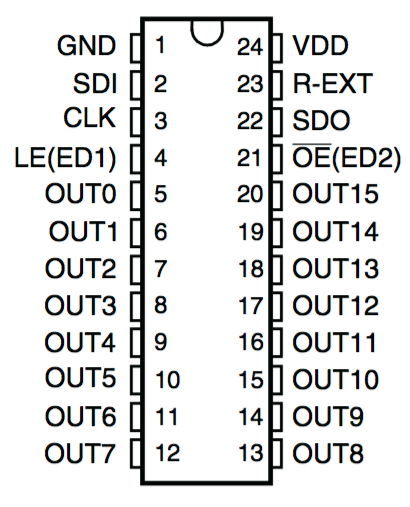
\includegraphics[scale=0.35]{./images/tlc-pins.png}
\caption{Pin layout of the TLC5927 LED driver}

\end{wrapfigure}

After quite some searching around, I decided to use the TLC5927 by Texas Instruments. It is
essentially a shift register with some extra features. Like every normal shift register, it has a
serial data input (SDI), a serial data output (SDO), and a clock pin (CLK). Additionally, there is
a latch pin (LE), which serves the purpose of only refreshing the state of the LEDs once all data
has been sent.

Furthermore, there is a pin called "output enable" (OE). If it is at GND, all LEDs are turned off,
and it's at \vdd, they are controlled by the data that the driver chip has received.

The most important feature, however, is the fact that each output is controlled by a constant
current driver. Without these, it would've been necessary to solder a resistor in series
with each individual LED, for a total of 480 resistors, 960 additional solder joints and a whole
lot of wasted board space. With the constant current drivers, however, I could use a single
resistor to set the current for all 16 LEDs attached to one chip.

Unlike most simple shift registers, the drivers' outputs are current sinks instead of current
sources. This will be important when selecting the LEDs: In order to control each colour separately
in an RGB LED, the cathodes have to be separated, while the anodes can be connected together.



\subsection{LEDs}

Like all the other parts, I ordered the LEDs from Digikey. Their website contains an excellent
tool, enabling the user to restrict the selection based on different criteria. My requirements
were the following:

\begin{itemize}

\item Colours: Red, green and blue

\item Current: 20 mA or more. Because the LEDs are within one pixel only $\frac{1}{100}$ of the
time, they are essentially pulse width modulated, reducing their effective brightness. In order to
still see the image clearly without darkening the room, they have to be bright enough.

\item Mounting type: Surface mount, so I can still use the other side of the board

\item Size: At most \SI{5}{\milli\meter} by \SI{5}{\milli\meter}, preferably smaller, but still
large enough to solder by hand

\item Diffused lens, so the colours mix well even when viewing the LED directly instead of using
it for illumination.

\end{itemize}

These requirements reduced the category "LED Indication - Discrete" from 18940 to 130 items.
From those remaining products, I chose the one that was cheapest in a quantity of 160. This
led me to an LED with the beautiful name CLVBA-FKA-CAEDH8BBB7A363.



\subsection{Capacitors}

A digital circuit like an LED driver can change its current consumption significantly within a
short amount of time. Because the connections to the power supply are relatively long, they have
a substantial parasitic inductivity. So when the IC suddenly needs more current because all its
LEDs have just been switched on, this current is not available instantly. Worse yet, if the LEDs
are on and then are turned off, the current can't immediately stop flowing and will induce
dangerous voltage spikes.

In order to prevent those two situations from happening, I used capacitors. Namely, each LED
driver has its own \SI{1}{\micro\farad}  ceramic capacitor.



\subsection{Motor}

In order for the whole device to rotate, I needed a motor. Luckily, I could salvage an appropriate
part from an old RC motor boat. It's a big and heavy brushed motor. The fact that it has a built-in
fan and was water-cooled in the boat leads me to think that its power output is much higher than
what I need.

Because of its high torque, I could attach the motor directly to the rotating shaft instead of
using gears or a belt drive. That way there are less moving parts and the motor can turn at a lower
rotational speed, both resulting in less wear and noise.



\subsection{Power Transmission}

To transmit power from the stationary power supply to the rotating part, I used slip rings. I made
a relatively simple version, consisting of two round pieces of copper sheet on the rotating end,
and two long pieces of copper sheet on the stationary part.

The slip rings must be able to transmit the current necessary to light all LEDs up at once.
Assuming that each LED needs 20 mA, this current is about 9.6 A. Additionally, there is a small
current draw by the microcontroller, but it will be negligible in comparison. Testing has shown
that the slip rings don't heat up noticeably when conducting 10 A for several minutes.

In practice, however, this current is not reached since the vast majority of pixels are
switched off when displaying a typical 3D image.

Because two pieces of copper sheet rubbing against each other aren't the most reliable electrical
connection, I used a \SI{2200}{\micro\farad} electrolytic capacitor to smooth out the supply
voltage. Even with it, I found that the pressure between the two copper conductors had to be quite
high for them to form a good contact.


\newpage
\section{Circuit Diagram}

\begin{figure}[h]
\vspace{4mm}
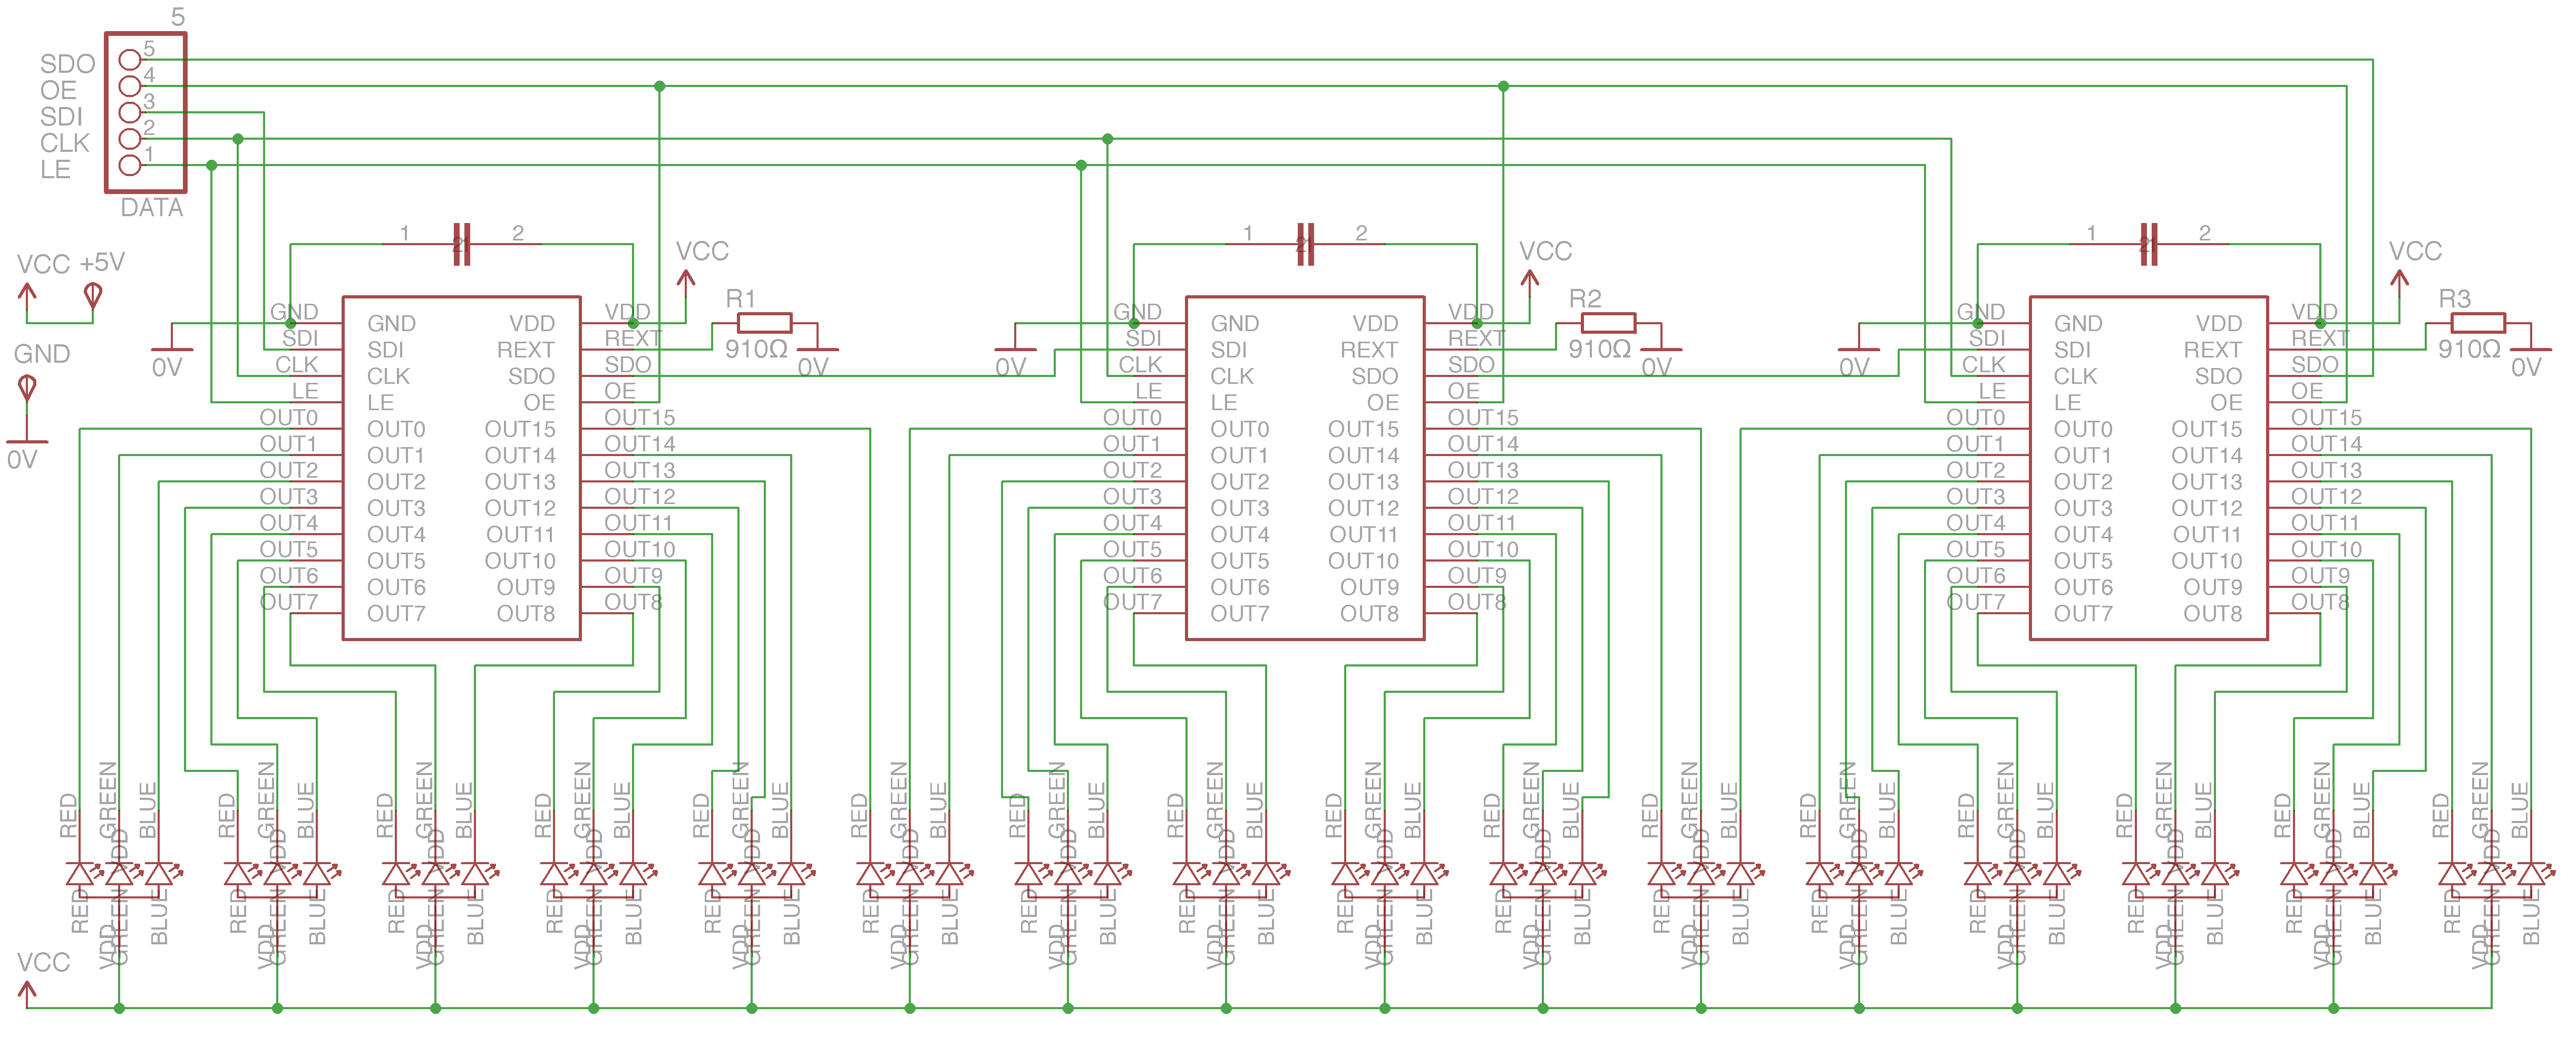
\includegraphics[width=\textwidth]{./images/schematic.png}
\vspace{-8mm}
\caption{The finished circuit diagram}
\vspace{6mm}
\end{figure}

The circuit diagram --- as well as the PCB layout --- were created in Eagle. Its free version is
limited to two-layer boards of sizes up to \SI{10}{\centi\meter} by \SI{8}{\centi\meter}, but
that's more than enough for my purposes.

In figure 2, the final version of the schematic is pictured. For the sake of simplicity and
readibility, the layout corresponds roughly to how the board will look.

I had to configure the footprints for the LED drivers and the LEDs by myself, which I did by
reading about the physical dimensions in the respective data sheet. For the resistors and
capacitors, Eagle had pre-built footprints which I could use.

\subsection{Data Interface}

For transmitting data to the LED drivers, I used a simple row of 5 pins. Two of those pins are the
data lines: The input is connected to the first chip's input, and the output comes from the last
chip's output. The rest of the pins (clock, output enable and latch enable) are control lines,
which go to all three chips simultaneously. The order of these connections was determined when
making the PCB layout.

\subsection{LED Drivers}

The LED drivers are arranged in a so-called daisy chain configuration, where the serial data output
of each chip is connected to the serial data input of the next chip. This is not only the case
within one board, but also between the different boards: The data output of one board is connected
to the next board's input. That way, all of the 30 LED drivers can be controlled by a single SPI
bus without anything like a chip select signal. To send data to the chips, the microcontroller
can simply send out 480 bit without interruption.

\def \iout {I\textsubscript{OUT}}
\def \rext {R\textsubscript{EXT}}

The external resistor which is connected to each LED driver sets the output
current. The following equation, taken from page 15 in the datasheet, describes the relation
between the output current (\iout) and the resistor's value (\rext):

% Lots of ugly hacks to have a non-italic font
\begin{ownmath}
\textrm{\iout} = 15 \cdot \frac{\SI{1.25}{\volt}}{\si{\rext}}
\end{ownmath}

Let's find out the resistance necessary for the output current to be \SI{20}{\milli\ampere}:

\begin{ownmath}
\textrm{\rext} = 15 \cdot \frac{\SI{1.25}{\volt}}{\SI{20}{\milli\ampere}} = \SI{937.5}{\ohm}
\end{ownmath}

The next smaller value within the E24 series is \SI{910}{\ohm}. By choosing this resistance, the
output current is \SI{20.6}{\milli\ampere}, which is close enough to the desired
\SI{20}{\milli\ampere}. I ordered 40 through-hole resistors of this value, because at the time I
had in mind to etch my own boards at home.


\subsection{LEDs}

The LEDs have their common anodes connected to \vdd. The cathodes are connected to a driver output
each, and are arranged red - green - blue (from left to right). Series resistors aren't needed
because the LED drivers handle current regulation.












\section{PCB Design}

\begin{figure}[h]
\vspace{4mm}
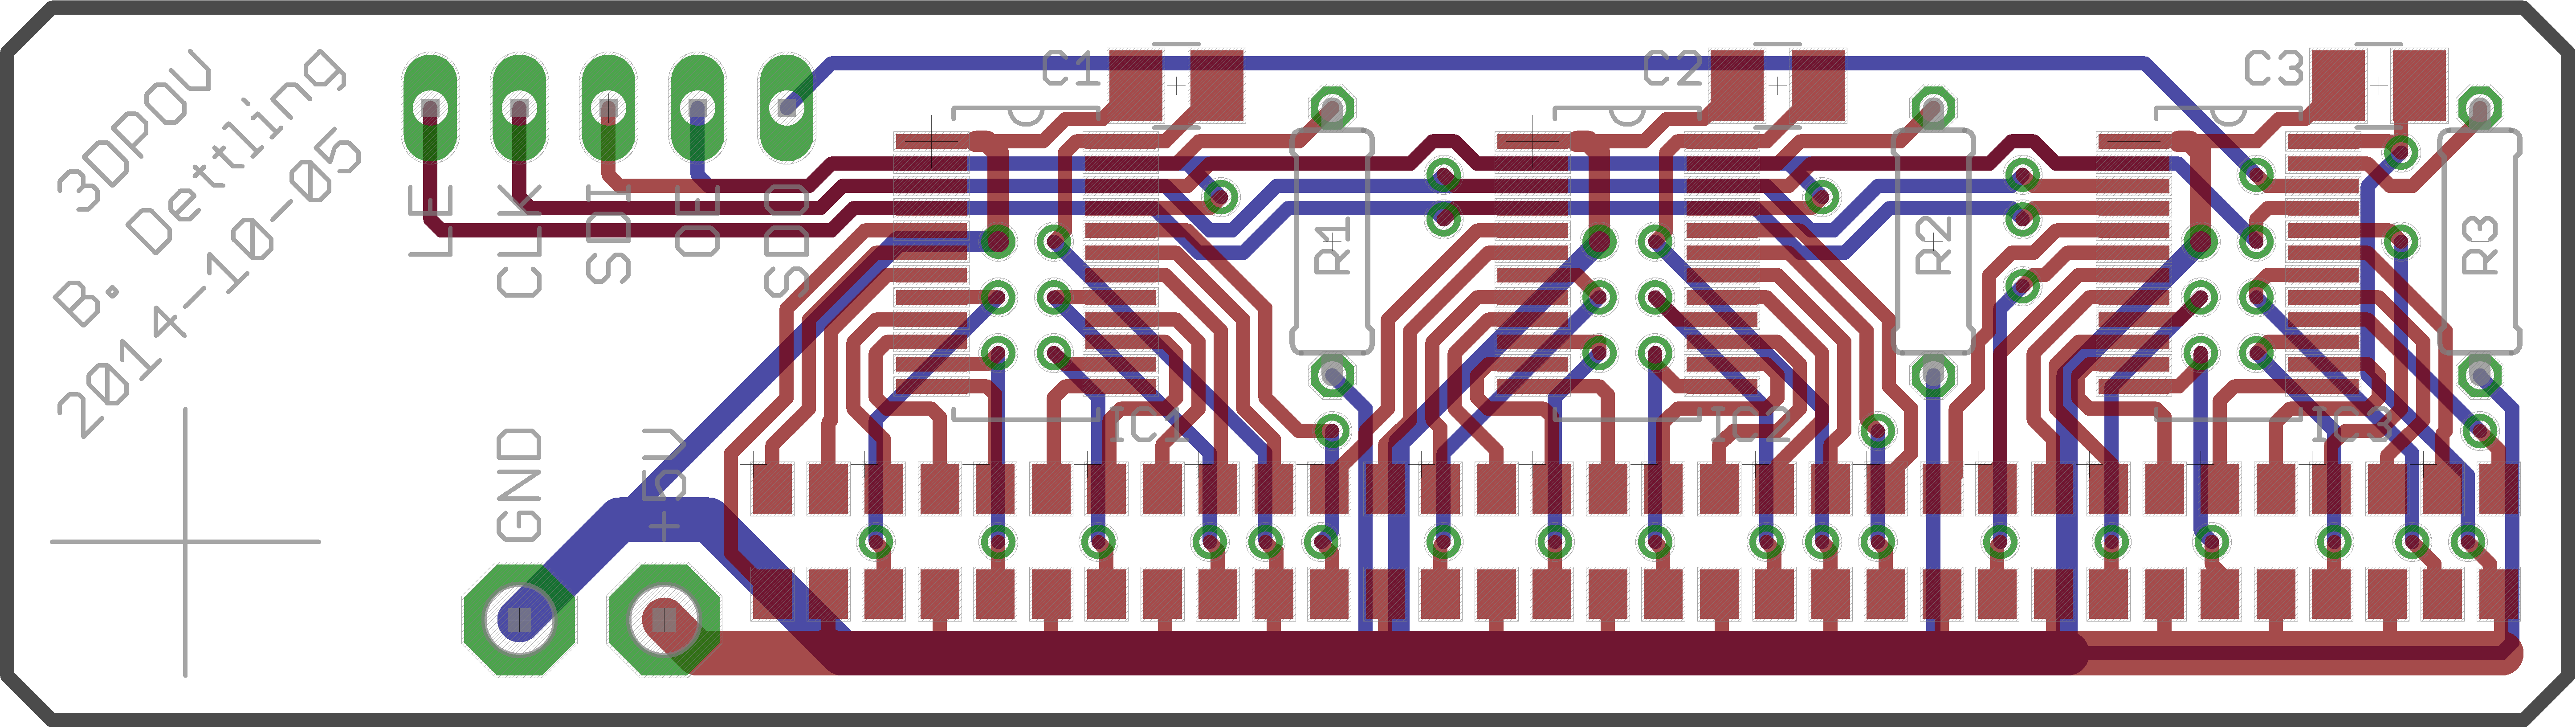
\includegraphics[width=\textwidth]{./images/board-layout.png}
\vspace{-6mm}
\caption{The PCB layout in Eagle. Red = upper copper layer, blue = lower copper layer,
green = vias, grey = silkscreen.}
\vspace{6mm}
\end{figure}

\subsection{General Remarks}

The defining factor for the board layout was the pin layout of the LED drivers. The outputs are all
at the bottom of the chip, while the data interface is at the top. This led me to the layout I have
now: the LEDs are in a row at the bottom of the board where they can be directly connected to the
driver outputs on the upper copper layer. The control lines are is routed on the back side of the
board behind the chips, with vias going to the front side to connect to each chip. The data lines
go straight from one chip to the next one on the upper copper layer, with the last output going
back to the board's data interface on the back side. The resistors are placed on the right side of
their respective driver IC, jumping across the data traces.

The supply lines are placed beneath the row of LEDs. Had I placed the supply on the upper edge of
the board, I still would've had to connect all the 16 anodes to \vdd. The driver chips, on the
other hand, only need one connection to \vdd and GND each, so by placing the supply lines at the
bottom of the board I have less traces running across the board vertically.

From a layout perspective, it would've made sense to put the GND line at the top of the board,
since the chips need one connection to that trace each, while the LEDs don't. However, I opted to
put both supply lines right above each other to reduce electromagnetic interference. If all the
LEDs are switched on suddenly and a lot of current starts to flow, a magnetic field builds up
quickly around the supply traces. This could induce bothering or even dangerous currents in the
surrounding electronics. By having the two supply lines close to each other, their magnetic fields
largely cancel each other out.


\subsection{Space-saving measures}

In order for the production to be as cheap as possible as well as to minimise the rotating mass, I
tried to make the boards as small as possible. Ultimately, I managed to bring the size down to
\SI{73}{\milli\meter} by \SI{21}{\milli\meter}.

In order to achieve this, but also to avoid large gaps between the pixels, I placed the LEDs as
close as possible to each other. The datasheet claims a width of \SI{2.8 \pm 0.2}{\milli\meter},
so I decided to place the LEDs at \SI{3}{\milli\metre} increments. On a grid of \SI{12.5}{mil},
the next larger distance is \SI{125}{mil}, which is equal to \SI{3.175}{mm}.

The connections to the cathodes of the red LED needs to pass by the other two cathodes, since
they're located on the lower side of the LED package. Because the LEDs are so close to each other,
the only option was to use the lower copper layer. The only place to go back to the upper copper
layer was right beneath the driver chips.

Initially, I had placed the decoupling capacitors right above the ICs. However, I could save a
small bit of vertical board size by placing them at an offset to the right. That way I could push
them down until where the pins begin, which is a bit further down than the edge of the chip itself.


\subsection{Thermal Considerations}

A positive side effect of placing some vias beneath the chip is their thermal conductivity, which
helps disspiate the chip's excess heat. The maximum power output of the chips --- when all the
attached LEDs are turned on --- is as follows:

\begin{ownmath}
\textrm{P\textsubscript{MAX}} = (\SI{5}{\volt} - \textrm{V\textsubscript{F}}) \cdot
\SI{20.6}{\milli\ampere\per output} \cdot \SI{16}{outputs} = \SI{780}{\milli\watt}
\end{ownmath}

V\textsubscript{F} is different depending on the colour of the LED, so I just used the average
value, which is \SI{2.633}{\volt}. The actual values are \SI{1.9}{\volt} for red and \SI{3}{\volt}
for green and blue.

A power output of \SI{780}{\milli\watt} is not to be underestimated on such a small PCB, and tests
have shown that that the boards do get quite hot when operated at full power. In reality, however,
the situation is much less severe because the LEDs are typically turned on only during a fraction
of the rotation. Furthermore, the quick rotation results in excellent air circulation, which aids
the dissipation of heat.









\chapter{Fabrication}

\section{Circuit Boards}

\subsection{Fabrication}

There's no shortage of firms who produce PCBs according to a custom layout. One of the cheapest
providers to ship small production runs within a reasonable timeframe and with good production
quality turned out to be OSHPark. They only produce in multiples of 3, so I ordered 12 instead of
10 (which I'd have done anyway to have some spare boards). I submitted my order on the 5th of
October 2014 and paid US\$ 47. Ten days later I received a message that the boards were finished,
and after another ten days of waiting they arrived at my doorstep.


\begin{figure}[h]
\vspace{3mm}
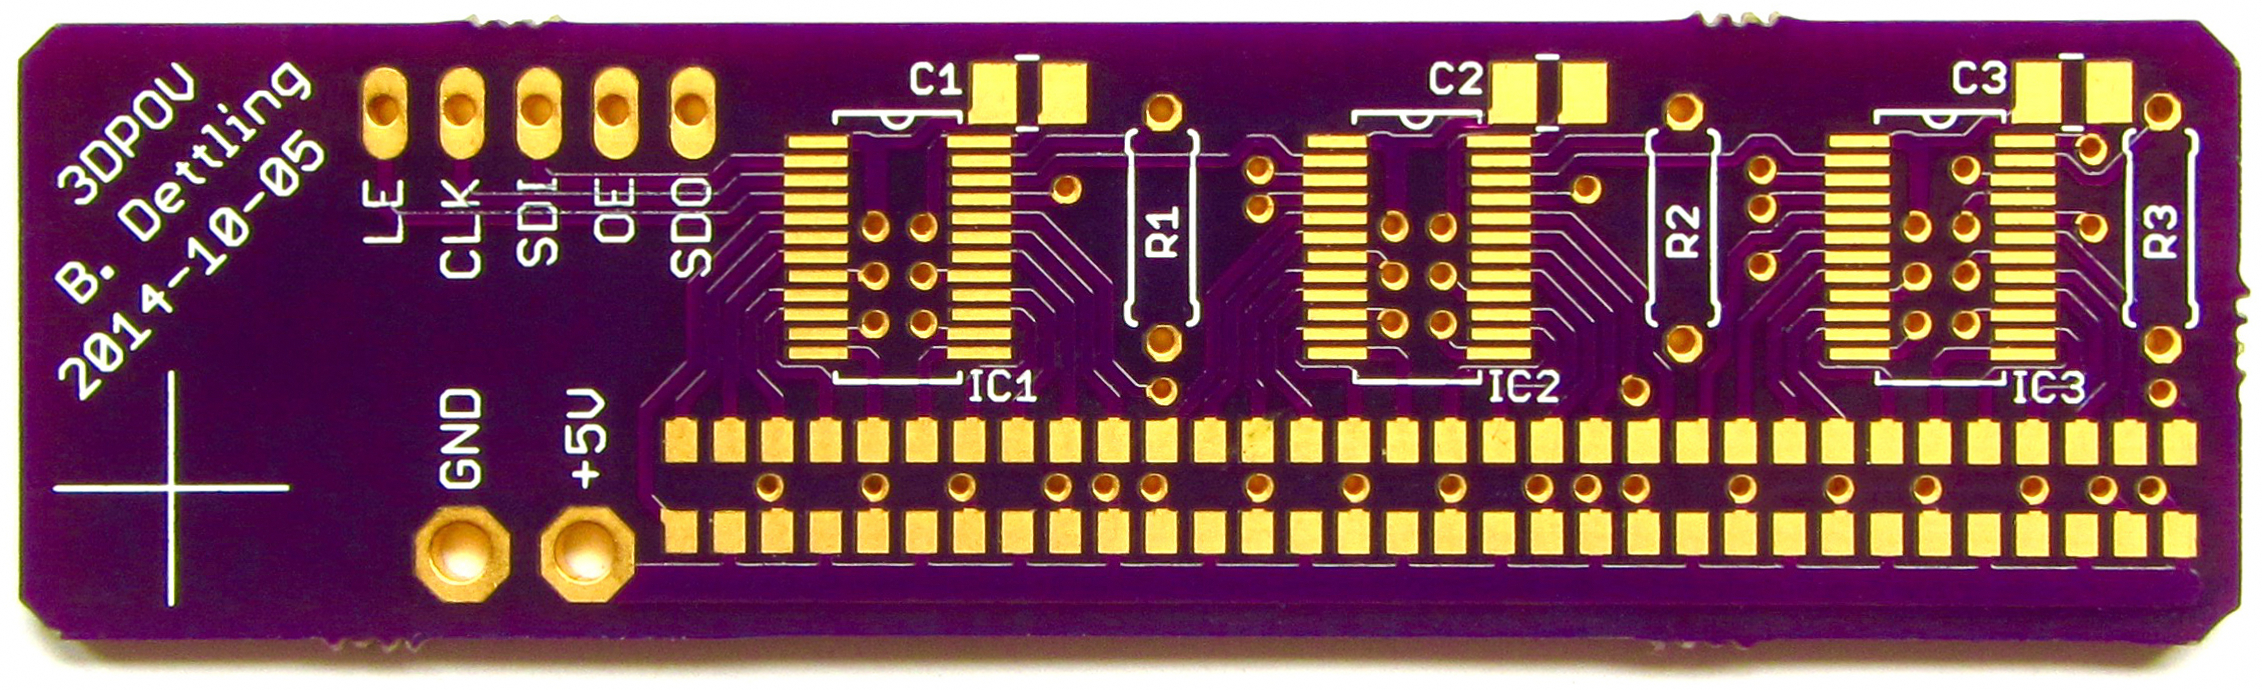
\includegraphics[width=\textwidth]{./images/board-finished.jpeg}
\vspace{-8mm}
\caption{A finished circuit board}
\end{figure}


\subsection{Assembly}

As soon as I got the boards in the mail, I started soldering the parts to them. I started with the
LEDs to avoid having to solder in the tight gap that would later be formed between the LEDs and
their driver chips. It took me two hours to solder the first board, but with increasing practice
the time for one row of LEDs got down to 25 or 30 minutes.

The chips were a lot easier to solder than the LEDs, despite the distance between the individual
pins only being \SI{0.635}{\milli\meter}. I could simply drown all the pins in solder, and then
wick away all the solder bridges. That way I could solder twelve pins within the blink of an eye.




\subsection {Testing and Debugging}

With the boards finished, I wanted to know whether or not they work. In order to find out, I wrote
a little program on the microcontroller to light the LEDs up in all possible colours consecutively.
It did not work at the first try, so I used an oscilloscope to see if data was being sent at all.
This was the case, the SPI library on the Teensy performed its task flawlessly.

It turned out that the culprit were the bad contacts. Instead of soldering the wires onto the board
and the microcontroller, I simply inserted them into the respective holes. This caused the
connection to have too much parasitic capacitance, and the signals (which were being sent at 4 MHz)
did not have time to propagate up to their destination.

I soldered the cables on properly and sure enough, the board worked as intended. I repeated this
procedure for all ten boards to see if they all worked as well as the first one, which wasn't the
case.

Because of reasons unbeknownst to me, one particular LED driver started turning on all of its LEDs
at a moderate brightness as soon as I powered it up --- even though no data was being sent at all.
At first I thought that the serial data input had a solder bridge pulling it up to \vdd, and
immediately sending a whole lot of 1's upon powering up the board. However, the data input pin was
not close enough to a positive supply line for this to be an issue. Additionally, there would have
to be a clock signal as well as a pulse on the latch pin for the LEDs to light up. I gave up and
assumed that the chip was faulty, and when I replaced it with a spare part everything worked
perfectly.

Apart from that, there were no major issues. I had a few LEDs which didn't light up when they
should have. One of them had a solder bridge between the common anode and the cathode of the red
LED, which made a voltage drop across the red LED impossible. Two were simply soldered on poorly
and weren't connected to the drivers at all. A few other LEDs didn't work and I found no obvious
issues. I replaced them with spares, which did the trick.


\section{Physical Assembly}


\subsection{Frame}

The frame was built out of beech wood strips with a square cross section and a side length of
\SI{1.5}{\centi\meter}. The baseplate is made out of plywood and has the dimensions
\SI{15}{\centi\meter} by \SI{15}{\centi\meter} by \SI{1}{\centi\meter}. On it, I mounted two
vertical wood strips with a length of \SI{20}{\centi\meter}, which were both stabilise by three
struts. A horizontal board, mounted to the vertical strips at a height of \SI{20}{\centi\meter},
holds the motor.

On the top of the two vertical strips I placed another strip to hold the shaft in its position.
A simple hole served as a bearing, which I later replaced with a plastic insert (kindly sponsored
by IGUS).

\subsection{Slip Rings}

In order to supply the rotating parts with electricity, I mounted a wooden disc right at the bottom
of the shaft. On both sides of that disc I glued on a round piece of copper sheet, which I then
connected to cables going up to where the electronics would later be.

On the stationary end, two long pieces of copper sheet serve as contacts. Because of their
spring-like properties, they exert a certain amount of pressure on the rotating disc.

Despite this, a considerable amount of pressure was necessary to form a good contact. The contact
pressure proved to be a primitive, but usable way of roughly adjusting the rotational speed of
the display. Sadly it's quite an inefficient approach: The motor uses a lot of current when
friction is applied to its load. It becomes noticeably warm after a few minutes of use, and
measurements on the current limiting resistors have shown that it draws about \SI{6.5}{\ampere} at
\SI{5}{\volt}.

This constant pressure, in addition to the fact that copper is quite a soft metal, results in
considerable wear on the slip rings. Luckily, the stationary ends can be replaced without much
hassle. The rotating part would be a pain to replace, but since wear is distributed across the
whole copper disc, it will be a long time before this needs to be done.


\subsection{Controller}

The microcontroller is mounted on another wooden disc, located a few centimetres above the slip
rings. It also hosts the hall sensor, which is used to measure the rotational speed and calculate
the position of the rotating part at any given moment. The corresponding magnet is mounted on a
piece of threaded rod, which itself is mounted on the same board as the motor.

Additionally, the \SI{2200}{\micro\farad} capacitor is located on the upper wooden disc. In the
end, this place has become a bit of a mess, especially with all the cables going up to the circuit
boards. Luckily this isn't visible while the apparatus is running.


\subsection{Circuit Boards}

The boards were already equipped with components, but what was missing was the hold to mount them
on the shaft. The diameter of this shaft is \SI{4}{\milli\meter}. In order to find a good hole
size, I drilled a few test holes on a spare board. A hole of \SI{4}{\milli\meter} was so small for
the boards to fit on the shaft, while \SI{4.5}{\milli\meter} was obviously too big. After
chamfering the top end of the shaft, the board with a \SI{4}{\milli\meter} hole just barely could
slide on the shaft. This tight fit proved to be advantageous, because torque can now be transmitted
reliably from the shaft to the boards, and they don't slide around.

There were two factors I had to carefully consider while arranging the boards:

\begin{itemize}
\item The boards had to be balanced out to minimise static and dynamic unbalance
\item The amount of boards obstructing other boards had to be minimal
\end{itemize}

In the end, I decided to arrange the boards in a double-spiral arrangement. This was the only
arrangement I could think of that (theoretically) has no static imbalance at all. Because each
board has another board on the exact opposite side of the shaft, there are five pairs of boards
where one board statically balances out the other. However, each pair has some dynamic inbalance
because the two boards aren't mounted at the same height. This could've been minimised by
alternating the order of boards between each pair. However, this wasn't necessary because the
vibrations were within reasonable bounds.

The visibility is not too bad either: On the viewer-facing half of the display, all LEDs are
constantly visible. On the backside, it is possible that one group of boards is right before the
other one, causing some layers of the image to disappear.


\chapter{Programming}

\section{Used Software}

The following program has been compiled with the Arduino IDE 1.0.6 and sent to the Teensy by the
Teensyduino 1.20 plugin. However, the most part of the program has been written in Sublime Text 2
with the stino plugin. This combination has a few advantages over simply using the Arduino IDE to
write all code, namely there's automatic code completion, support for several cursors, and a
search-and-replace function with regex suport. I installed and used these programs on Mac OS 10.9
and later 10.10.

\section{Timing}

\subsection{Theory}

In order for the image to stay still despite the rotational speed not being completely constant,
the frequency of LED refreshed must be constantly adjusted based on the rotational period. Because
there are 100 pixels per revolution, the time to display one pixel must be $\frac{1}{100}$ of the
rotational period.

This value can be measured easily by using the hall sensor. By dividing this value by 100, we can
obtain the duration of one pixel for the current speed. If the rotational speed changes, that's a
bit of a problem: The measured value is from the previous rotation, but in the current rotation,
the device already turns slightly faster. This causes the image to be slightly warped right after
powering up the display. However, once it has reached temrminal velocity, this effect is no longer
noticeable, because now the subsequent rotations have about the same period.

\subsection{Implementation}

This behaviour is implemented with an interrupt that runs each time the magnet is detected (i.e.
after each rotation). Within that interrupt, several things happen:

First, we read a variable called \texttt{sinceMagnet}. As its name says, it keeps track of
the number of microseconds since the last time the magnet was detected. It's of the special type
\texttt{elapsedMicros}, which means that it's automatically incremented each microsecond. This
value is divided by 100 and stored in \texttt{microsPerPixel}, where it represents the amount of
time that any given pixel should be displayed for.

This variable is now reset to 0 to start the new rotation. The same is done to another
variable, \texttt{nextPixelMicros}. It contains the next point in time when the pixels
should be refreshed, with respect to the start of the rotation (which just happened).

In the main loop of the program, this variable is continuously compared to \texttt{sinceMagnet}. If
sinceMagnet is bigger, the LEDs are refreshed by calling \texttt{sendData}. Within that function,
\texttt{nextPixelMicros} is incremented by \texttt{microsPerPixel}, causing the program to wait for
the display to turn another $\frac{1}{100}$ of a full circle. After that, it'll display the next
pixel.

The implementation of the described behaviour can be found in the appendix, where the whole source
code is to be found. Specifically, what I've just talked about is contained in the
\texttt{timerUpdate} function, as well as in the main \texttt{loop}.


\section{Data storage and display}

The previously mentioned function \texttt{sendData} needs to be able to know which bytes to send
based on one parameter, which is the current angle of of the display. In this section, I will
explain how I achieved this.

To save the image on the microcontroller, I used a simple three-dimensional array containing $100
\cdot 10 \cdot 6$ bytes of data. The first index stands for the angle of a pixel in hundredths of
a circle, the second index corresponds to the height and the third one describes the position of
each byte on a row of LEDs. Because there are 48 LEDs per row, 6 bytes can be used to describe the
row's state without wasting any storage space. The only way to be more efficient in terms of
storage would be to compresss data, which would require significantly more computing power.

Because the PCBs are not right above each other, the data that is being sent out in one refresh
don't correspond to the pixels that are above each other in the image. In order avoid having to
account for the angular offsets of each board while creating an image, I made the program do that
work automatically.

Each pair of two boards are mounted on the exact opposite side, making the angle between them
\SI{180}{\degree} or 50 pixels. Each subsequent pair is additionally rotated by \SI{28.8}{\degree}
which is equivalent to 8 pixels.

The program accounts for this arrangement by using a simple for loop. It iterates over five pairs
of boards. At its start, the program calculates the angle and height of the first board based on
the control variable. After the data has been sent, it then moves to the second board by adding 50
to the angle and incrementing the board counter, and feeds the second board with data too.

After these two additions, the angle value will go over 99 in many cases, which is the highest
possible array index. Since the pixel at position $100+n$ is the same as the one at position $n$, I
can pervent causing undefined behaviour by applying a modulus 100 operator to the angle value
before using it to access the array.


\section{Miscellaneous}

While the program works the way it is described above, there are a few small things that I managed
to further improve.

Because I selected the position of the boards with respect to the hall sensor arbitrarily, the
image was turned around. To fix that, I added a constant value to all angle values, so now the
first pixel is displayed exactly at 0° instead of whereever the hall sensor detects the magnet.

Whenever I started up the program, it started displaying the first pixel. It even did so when I
connected the Teensy to my laptop via USB. This was dangerous because neither the Teensy nor the
laptop's USB port can handle a lot of current, and if more than a handful of LEDs were switched on,
the Teensy could've been damaged.

To fix this I added a boolean variable called \texttt{running}, which is set to \texttt{false} by
default and only flipped when the magnet is first detected. That way the program only starts
running if the display is actually rotating, at which point we can be sure that power is supplied
through the slip rings rather than the USB port.

The images displayed were constantly jittering around instead of staying still like they should. It
took me a long time to find the source of this bug, but I managed to fix it in time for the swiss
national competition organised by "Swiss Youth in Science".

The problem was that sometimes, the magnet was detected while \texttt{sendData} was still running.
Because the hall sensor's interrupt had a higher priority than the timer interrupt I had used to
send data, control was immediately given to the former. The \texttt{timerUpdate} function was
executed normally, resetting \texttt{currentPixel} to zero and reading out the duration of the last
rotation. However, after that, control was given bach to the \texttt{sendData} function. At the end
of that function, \texttt{currentPixel} was incremented by one. That way, the \texttt{currentPixel}
variable already had a value of one when it should've stayed at 0. For the entirety of the next
rotation, \texttt{currentPixel} was off by one, resulting in the image quickly turning by
\SI{3.6}{\degree}.




\chapter{Operation}

\section{Power Supply}

Initially I had planned to supply the PCBs with \SI{5}{\volt}. However, the Teensy sends its
signals at \SI{3.3}{\volt}. The driver chips, on the other hand, only read a logical high when a
signal is over $0.7 \cdot \textrm{\vdd}$. At \SI{5}{\volt}, this value would be \SI{3.5}{\volt}.
So I tried powering the boards with only \SI{3.3}{\volt}, and everything worked perfectly. Better
yet, the boards weren't getting as hot anymore.

According to the manufacturer, the Teensy needs at least \SI{3.7}{\volt} to operate, presumably
because it uses a linear regulator to get a stable voltage ov \SI{3.3}{\volt}. However, there were
no problems when I started using \SI{3.3}{\volt}. Even though the regulator probably reduces that
voltage to less than \SI{3}{\volt}, the processor still runs at its full clock speed of
\SI{96}{\mega\hertz}.

Unfortunately, the PC power supply which I used for the project broke down. As I later found out,
the culprit was the motor consuming too much current. At that time, I didn't use any series
resistance to limit the current flowing through the motor, which I powered with \SI{3.3}{\volt}.
This has caused the inrush current to be greater than what the power supply could handle.

To remedy this, I used a pair of long, thin wires to connect to the motor to provide some
resistance. I later replaced these with two \SI{150}{\milli\ohm} power resistors. Now there are two
ways to power the motor: I can use \SI{5}{\volt} and connect the resistors in series for a total
resistance of \SI{300}{\milli\ohm}, or I can power it with \SI{3.3}{\volt} and connect the
resistors in parallel, resulting in a resistance of \SI{75}{\milli\ohm}. The latter method is more
efficient, but it causes the acceleration at startup to be slower.


\section{Mechanical Problems}

Because the slip rings weren't fixed in their position, they could slide out of their slots after
a few minutes of operation. I fixed this issue by mounting a small wooden board onto these slots
(perventing lateral movement), and routing the cables going from the power supply to the slip rings
through two holes in that board (perventing lengthwise movement).

The boards weren't exactly aligned at the \SI{28.8}{\degree} that I specified. This caused the
image to be displayed crookedly: Pixels that should've been right above each other were shifted
sideways by a small distance. Whenever I adjusted the boards, they would be misaligned again after
using the display for some time. To fix this, I aligned them correctly one last time and used
enough solder on the power cables running through the boards for them to form a solid connection.

The bolt nut that held the motor in place started coming loose because of the vibrations. To
pervent that from happening again, I used a second nut and tightened it against the first one.


\chapter{Conclusions}

\section{Possible Improvements}

\subsection{Controller and Data Transmission}

The Teensy 3.1 is currently mounted quite loosely on its wooden disc. A piece of wire goes through
two unoccupied contacts as well as through two holes in the disc. In addition, the cables forming
the SPI bus aren't laid out neatly at all; many are too long and don't take the direct route.

This situation could be improved by replacing the upper wooden disc with another printed circuit
board. All connections could be routed elegantly on the PCB, and the SPI interfaces could be
formed by two ribbon cables. The hall sensor could be properly soldered on instead of fixing it in
place using hot glue.

Between the individual LED boards, ribbon cables could also be considered. However, the only
connections that always go to the board right above are CLK, LE and OE, while the serial data
inputs and outputs have to be connected to the board on the opposite side. These connections would
still have to be formed by individual cables.


\subsection{Slip Rings}

Because the slip rings are quite rough and not completely horizontal, a lot of pressure is needed
to form a consistent contact. This leads to high friction between the two contacts, which then
results in quick wear as well as a lot of friction.

The main reason why the display is not energy efficient at all are the slip rings. At the start of
the project, I had the idea of using a \SI{3.5}{\milli\meter} phone connector to transmit power.
However, I abolished that plan because of two reasons. Firstly, I had concerns that such a small
connector would have trouble conducting the maximum current of \SI{10}{\ampere}. This would most
likely not have been a problem, since only a small part of all pixels are turned on in a typical
image, which causes the average current to be a small fraction of the maximum value.

The second problem would've been the difficulty of mounting a phone connector on the display. I
would've had to place it at the end of the shaft, where it would've also served as a bearing. In
order to minimise the forces acting upon the plug, it would've had to be mounted exactly in the
center of the shaft. I couldn't come up with a solid way to connect both of the phone plugs' ends
to the display.

A much more elegant solution would've been to use induction to transfer power. By having a
stationary and a rotating coil close together, I could've passed a high-frequency alternating
current through the stationary one, causing current to flow in the rotating one as well. The
advantages of such an approach would be substantial: The bearings would be the only contact point
between the rotating and stationary part, causing friction to be minimal. I could've also
completely eliminated the annoying, broadband noise currently emitted by the slip rings.

I didn't implement wireless power transfer because I felt like the extra work wasn't worth it,
especially considering this was a prototype. If I wanted to produce this display en masse,
inductive power transfer would definitely be the way to go as it's the only way to make the
display somewhat quiet.


\subsection{Motor}

I decided to drive the display directly without any kind of gear reduction because that was the
simplest solution. I only could do so because the motor was strong enough. Unfortunately, it
consumes a substantial amount of current.

If I wanted to sell my display commercially, I'd use a smaller motor, drive it at a higher
rotational speed and gear it down. To save energy, I would also implement one of the above
imporvements concerning power transmission.


\section{Future Outlook}

\subsection{Animated images}

Something I had in mind since the beginning of this project were animated images. The Teensy 3.1
has \SI{256}{\kilo\byte} of memory, which would fit 42 images of \SI{6}{\kilo\byte} each. This
corresponts to roughly a second of playback. In order to display longer animations, there are
several workarounds: Instead of showing one image that spans the entirety of the rotation, I can
instead only save an image that is 25 pixels and display it four times.

In order to get around the limit of flash memory, external storage would be necessary. Even with
only \SI{1}{\giga\byte}, I could save 166666 frames, thus removing any practical limit in terms of
playback time.

\subsection{Interactive Programs}

It would be interesting to not only display predefined images, but to actually run a program that
can respond to user input, like a video game. In order to communicate with the external world, a
wireless interface would be necessary. Readily available solutions include small WLAN or bluetooth
modules, or the transmitters and receivers commonly used in radio-controlled aircraft.

\subsection{Applications}

Because of the low resolution and colour depth, the high level of noise, quick wear and the
inability to send images to the display while running, this display is not suited as a replacement
for your everyday computer or TV screen. However, these problems can all be fixed completely or
partially, so that there could one day exist a version of my display which is actually suitable
for the above purposes.

One domain where I could imagine a display like mine being especially useful is advertising.
Because most people haven't ever seen such a display before, it would be an immediate eye-catcher
in the display window of any business.

Another possibility would be video games. Although the limited resolution and computing power
would make it difficult to run the newest games, 3D version of classics like Pong, Snake or a
simple platform game would be worth a shot.






























\end{document}
